\documentclass[12pt, a4paper]{article}

\usepackage[utf8]{inputenc}
\usepackage{amsmath}
\usepackage{graphicx}
\usepackage{float}
\usepackage{pgfplots}
\usepackage{tikz}
\usepackage{pgfplotstable}
\pgfplotsset{compat=1.18}
\usepackage{titlesec}
\usepackage{enumitem}

\usepackage[table]{xcolor} 
\usepackage{booktabs}      
\usepackage{tcolorbox}     
\usepackage{geometry}      
\usepackage{array}  
\usepackage{subcaption}

\usepackage[labelfont=bf, textfont=it, skip=10pt]{caption}

\geometry{a4paper, margin=2cm}

\definecolor{MainBlue}{RGB}{41, 128, 185}   
\definecolor{DarkBlue}{RGB}{44, 62, 80}     
\definecolor{LightGray}{RGB}{245, 247, 250} 

\renewcommand{\arraystretch}{1.6} 
\setlength{\tabcolsep}{12pt}  
% ---------------------------------------------------------

% ---------------------------------------------------------
% ---------------------------------------------------------
% ---------------------------------------------------------
\usepackage{fancyhdr}
\pagestyle{fancy}
\fancyhf{} 

\geometry{top=2.5cm, bottom=2.5cm, includehead}
\setlength{\headheight}{28pt} 

\lhead{
    \begin{minipage}[b]{0.25\textwidth}
        \includegraphics[height=0.7cm]{logo.png} 
    \end{minipage}
}

\rhead{
    \begin{minipage}[b]{0.7\textwidth}
        \raggedleft
        {\fontsize{9.5}{11}\selectfont\bfseries\color{DarkBlue} National Higher School of Autonomous Systems Technology} \\[1pt]
        {\fontsize{8.5}{10}\selectfont\bfseries\color{MainBlue} Strength of material LAB -- Bending test}
    \end{minipage}
}

\renewcommand{\headrule}{%
    \vspace{1pt}%
    \hrule width \headwidth height 1pt %
}

\rfoot{\small\thepage}

\begin{document}
% ---------------------------------------------------------
% ---------------------------------------------------------

\thispagestyle{plain}

\begin{center}
    {\fontsize{13}{15}\selectfont\bfseries\color{DarkBlue} National Higher School of Autonomous Systems Technology} \\
    \vspace{0.1cm}
    {\fontsize{10}{12}\selectfont\color{MainBlue} Preparatory Cycle -- Second Year} \\
    
    \vspace{1.2cm}
    
    \begin{tcolorbox}[
        colback=MainBlue!5,
        colframe=MainBlue,
        arc=3mm,
        boxrule=1.2pt,
        halign=center,
        valign=center,
        width=0.95\textwidth,
        top=0.3cm, bottom=0.3cm,
        fontupper=\Large\bfseries\color{DarkBlue}
    ]
        LAB REPORT 2: Bend Testing of Beams
    \end{tcolorbox}
    
    \vspace{0.8cm}
    
    \noindent
    \begin{minipage}{0.9\textwidth}
        \centering
        {\small\bfseries\color{DarkBlue} Prepared by:} \\[0.15cm]
        \begin{tabular}{cc}
            {\small\bfseries Khaled Baroud} & \hspace{2cm} {\small\bfseries Bouchra Benarba}
        \end{tabular} \\
        \centering
        {\small\bfseries\color{DarkBlue} Group:} \\[0.15cm]
        \centering
        {\small\bfseries\color{DarkBlue} LA4} \\[0.15cm]
    \end{minipage}
    
    \vspace{0.5cm}
    \color{gray}\vline height 0.4pt width 0.8\textwidth \color{black}
\end{center}

\vspace{0.4cm}

% ---------------------------------------------------------
% ---------------------------------------------------------
\pagestyle{fancy}

\titleformat{\section}
{\fontsize{12}{14}\selectfont\bfseries\color{DarkBlue}}
{\thesection}{1em}{}

\section{Introduction}
\noindent In this laboratory session, we successfully conducted a practical bend testing investigation to deeply explore how materials deform under structural loading conditions. Through this hands-on experience, we gained a comprehensive understanding of the mechanical principles behind flexural stress and familiarized ourselves with the operation of the Materials Testing Machine (MTM) used to apply precise forces. The experiment itself consists of a standard three-point bending setup designed to evaluate the behavioral differences between ABS beams configured in both I-shape and H-shape profiles. By capturing real-time data, we were able to evaluate how cross-sectional orientations alter a component's stiffness and flexural modulus, while validating our empirical findings against theoretical calculations and numerical software simulations.

\section{Objectives}
The core milestones intended to be achieved through this experimental work are to:
\begin{itemize}[noitemsep, topsep=2pt]
    \item \textbf{Machine \& Setup Mastery:} Learn how to properly configure and operate the material testing apparatus.
    \item \textbf{Geometry \& Inertia Analysis:} Investigate how the beam's cross-section orientation affects its bending resistance.
    \item \textbf{Data Interpretation:} Process raw experimental data to plot force-displacement curves and determine stiffness.
    \item \textbf{Property Evaluation:} Estimate the experimental flexural modulus of the ABS material.
    \item \textbf{Three-Way Comparison:} Validate physical test results against RDM7 numerical simulations and theoretical formulas.
\end{itemize}

\clearpage
% ---------------------------------------------------------
% Part 1 : Theoretical
% ---------------------------------------------------------
\begin{tcolorbox}[
    colback=MainBlue!5,
    colframe=MainBlue,
    arc=3mm,
    boxrule=1pt,
    halign=center,
    fontupper=\Large\bfseries\color{DarkBlue}
]
Part 1 : Theoretical
\end{tcolorbox}
\vspace{0.3cm}
\noindent This table was filled in based on the theoretical data provided and the dimensions measured during the laboratory work, namely:
\begin{itemize}[noitemsep, topsep=4pt]
    \item \textbf{Total Beam's Length ($L$):} $60\text{ mm}$
    \item \textbf{Total Height of the $I$-section ($h$):} $10.1\text{ mm}$
    \item \textbf{Flange Length ($b$):} $6.4\text{ mm}$
    \item \textbf{Web Thickness ($e_w$):} $1.6\text{ mm}$
    \item \textbf{Flange Thickness ($e_f$):} $1.0\text{ mm}$
\end{itemize}
where these data represent the theoretical values that we will compare with the experimental values.
\vspace{0.4cm}
\begin{table}[H]
\centering
\rowcolors{2}{LightGray}{white}
\begin{tabular}{p{5cm} p{5.2cm} p{5.2cm}}
\toprule

\rowcolor{MainBlue}
\textcolor{white}{\textbf{Properties}} &
\textcolor{white}{\textbf{I-beam (bending about the $z$ axis)}} &
\textcolor{white}{\textbf{H-beam (bending about the $y$ axis)}} \\

\midrule

Beam's length [mm] & 60 & 60 \\

Cross sectional area [mm$^2$] & 25.6 & 25.6 \\

Moment of inertia [mm$^4$] & 328.53 &  46.42 \\

Flexural modulus [GPa] & 2.5 & 2.5 \\

$F/\Delta x$ [N/m] & 182,518 & 25,790 \\

\bottomrule
\end{tabular}

\caption{Theoretical geometric and mechanical properties of the beams.}
\label{tab:theoretical_properties}
\end{table}

\vspace{0.3cm}

\newpage
% ---------------------------------------------------------
% ---------------------------------------------------------
\begin{tcolorbox}[
    colback=MainBlue!5,       
    colframe=MainBlue,        
    arc=3mm,                  
    boxrule=1pt,              
    halign=center,            
    fontupper=\Large\bfseries\color{DarkBlue} 
]
Part 2 : Numerical Analysis
\end{tcolorbox}
\vspace{0.2cm}

% ---------------------------------------------------------
% ---------------------------------------------------------
\noindent\textcolor{DarkBlue}\;\;We performed simulations in the RDM7 software using the measured dimensions and the mechanical properties of the beam.
\begin{figure}[H]
    \centering
    \includegraphics[width=0.75\linewidth]{image.png}
    \caption{RDM7 visualization}
    \label{fig:placeholder}
\end{figure}

\vspace{0.2cm}


% ---------------------------------------------------------
% ---------------------------------------------------------
\begin{table}[h!]
\centering
\rowcolors{2}{LightGray}{white} 
\begin{tabular}{lcc}
\toprule 
\rowcolor{MainBlue} 
\textcolor{white}{\textbf{Properties}} & 
\textcolor{white}{\textbf{I-beam ($z$-axis)}} & 
\textcolor{white}{\textbf{H-beam ($y$-axis)}} \\ 
\midrule 

Cross sectional area $[\text{mm}^2]$ & 

26& 

26\\ 

Moment of inertia $[\text{mm}^4]$ & 

300& 

32\\ 
\bottomrule 
\end{tabular}

\caption{Geometric properties of the cross-sections obtained via RDM7.}
\end{table}

\vspace{0.8cm}

% ---------------------------------------------------------

% ---------------------------------------------------------


\vspace{0.5cm}

% ---------------------------------------------------------

% ---------------------------------------------------------
\begin{table}[H]
\centering
\rowcolors{2}{LightGray}{white}
\begin{tabular}{cc c cc}
\toprule
\rowcolor{MainBlue}
\multicolumn{2}{c}{\textcolor{white}{\textbf{I-beam ($z$-axis)}}} & 
\cellcolor{white} & 
\multicolumn{2}{c}{\textcolor{white}{\textbf{H-beam ($y$-axis)}}} \\
\cmidrule{1-2} \cmidrule{4-5} 

\rowcolor{MainBlue!80} 
\textcolor{white}{\textbf{Force [N]}} & \textcolor{white}{\textbf{Displacement [mm]}} & 
\cellcolor{white} & 
\textcolor{white}{\textbf{Force [N]}} & \textcolor{white}{\textbf{Displacement [mm]}} \\ 
\midrule

50  & 
    0.003164 & & 50  & 0.02306 
    \\ 
100 & 
    0.006328 & & 100 & 0.04613
    \\ 
150 & 
    0.009493 & & 150 & 0.06919
    \\ 
\bottomrule
\end{tabular}

\caption{Numerical displacement values corresponding to different force levels.}
\end{table}


\clearpage

% ---------------------------------------------------------
% Part 3 : Experimental
% ---------------------------------------------------------

\begin{tcolorbox}[
    colback=MainBlue!5,
    colframe=MainBlue,
    arc=3mm,
    boxrule=1pt,
    halign=center,
    fontupper=\Large\bfseries\color{DarkBlue}
]
Part 3 : Experimental
\end{tcolorbox}
\vspace{0.6cm}
\noindent\textcolor{DarkBlue} \;\; After conducting the column bending test using the MTM and its software, force and displacement data were obtained. This data was used to perform a linear curve fit and determine the slope, which represents stiffness. The table below was also completed. 
\vspace{0.6cm}

\begin{figure}[H]
    \centering
    \begin{subfigure}{0.5\textwidth}
    \includegraphics[width=0.85\linewidth,height=5cm]{20260510_135601_(0).jpg}
    \label{fig:placeholder}
    \end{subfigure}%
    \begin{subfigure}{0.5\textwidth}
\centering
\includegraphics[width=0.85\textwidth,height=5cm]{20260510_135552_(0).jpg}
\end{subfigure}
\caption{Bending test}

\end{figure}

\vspace{0.6cm}

% ---------------------------------------------------------
% ---------------------------------------------------------
\begin{table}[H]
\centering
\rowcolors{2}{LightGray}{white}
\begin{tabular}{cccc}
\toprule

\rowcolor{MainBlue}

\multicolumn{4}{c}{\textcolor{white}{\textbf{$F/\Delta x \ [N/m]$}}} \\

\midrule

\rowcolor{MainBlue!80}
\textcolor{white}{\textbf{Beam}} &
\textcolor{white}{\textbf{Length [mm]}} &
\textcolor{white}{\textbf{Test 1}} &
\textcolor{white}{\textbf{Value with uncertainty}} \\

\midrule

I & 60 & 151,429.56 & 151,429.56 \\

H & 60 & 24,686.77 & 24,686.77 \\

\bottomrule
\end{tabular}

\caption{Experimental stiffness values obtained for the tested beams.}
\end{table}
\vspace{0.3cm}
\textbf{Note:} The I-beam is stiffer than the H-beam because \(I_z\) is larger than \(I_y\). A greater moment of inertia leads to smaller deflection under the same force.
\vspace{0.4cm}
\titleformat{\section}
{\fontsize{13}{15}\selectfont\bfseries}
{\thesection}{1em}{}
\section{Flexural Modulus Calculation}
Based on the theoretical formulas, we filled out the table below and calculated the flexural modulus. 
\vspace{0.1cm}
For a three-point bending test, the relationship between load and deflection is:

\begin{equation}
\delta = \frac{FL^3}{48EI}
\end{equation}

Rearranging for flexural modulus:

\begin{equation}
\boxed{E = \frac{L^3}{48I} \times \frac{F}{\Delta x}}
\end{equation}

where:
\begin{itemize}
    \item $E$ = Flexural modulus (Young's modulus) [Pa]
    \item $L$ = Span length between supports = 60 mm
    \item $I$ = Second moment of area [m$^4$]
    \item $F/\Delta x$ = Measured stiffness [N/m]
\end{itemize}

% ---------------------------------------------------------
% ---------------------------------------------------------
\begin{table}[H]
\centering
\noindent
\rowcolors{2}{LightGray}{white}

\begin{tabular}{p{4cm} p{5cm} p{5cm}}

\rowcolor{MainBlue}
\textcolor{white}{\textbf{Properties}} &
\textcolor{white}{\textbf{I-beam (bending about the $z$ axis)}} &
\textcolor{white}{\textbf{H-beam (bending about the $y$ axis)}} \\

\midrule

Beam's length [mm] & 60 & 60 \\

Material & ABS & ABS \\

$F/\Delta x \ [N/m]$ & 151,429.56 & 24,686.77 \\

Flexural modulus & $3.47\text{ GPa}$ & $2.27\text{ GPa}$ \\

\bottomrule
\end{tabular}

\caption{Experimental analysis of the beam properties.}
\end{table}


\begin{tcolorbox}[
    colback=MainBlue!5,
    colframe=MainBlue,
    arc=3mm,
    boxrule=1pt,
    halign=center,
    fontupper=\Large\bfseries\color{DarkBlue}
]


\newpage
Part 4 : Analysis and Comparison
\end{tcolorbox}
% ---------------------------------------------------------
% ---------------------------------------------------------
\vspace{0.3cm}
\begin{enumerate}[label=\textbf{\arabic*.}, leftmargin=*]
    \item \textbf{Plot the theoretical, numerical, and experimental force-displacement curves. What do you observe?} \\
        \begin{enumerate} \item \textbf{Theoretical Force-Displacement Curves} \\
        
    % ---------------------------------------------------------
% ---------------------------------------------------------
\noindent To construct the theoretical force-displacement curves, we utilize the fundamental linear elastic relationship derived from Hooke's Law:
\begin{equation}
    F = k_{th} \cdot \Delta x \implies \Delta x = \frac{F}{k_{th}}
\end{equation}
where $F$ represents the applied bending force, $\Delta x$ is the resulting beam deflection (displacement), and $k_{th}$ is the theoretical stiffness ($F/\Delta x$) calculated analytically in Table 1. 

\noindent Since the material behaves in a perfectly linear elastic manner under these load configurations, the curves are straight lines passing through the origin $(0,0)$. To ensure a direct and clear comparison with the subsequent numerical and experimental parts, the displacement values $\Delta x$ were computed at three distinct force levels ($50\text{ N}$, $100\text{ N}$, and $150\text{ N}$) by converting the stiffness from $[\text{N/m}]$ to $[\text{N/mm}]$ as follows:
\begin{itemize}[noitemsep, topsep=3pt]
    \item \textbf{I-beam ($z$-axis):} With a theoretical stiffness of $k_{th} = 182.518\text{ N/mm}$, the calculated deflections are $0.2739\text{ mm}$, $0.5479\text{ mm}$, and $0.8218\text{ mm}$ respectively.
    \item \textbf{H-beam ($y$-axis):} With a significantly lower stiffness of $k_{th} = 25.790\text{ N/mm}$ due to its cross-sectional orientation, the corresponding deflections expand linearly to $1.9387\text{ mm}$, $3.8775\text{ mm}$, and $5.8162\text{ mm}$.
\end{itemize}

\vspace{0.4cm}

\begin{figure}[H]
    \centering
    \begin{tikzpicture}
        \begin{axis}[
            width=0.95\textwidth,
            height=8.5cm,
            xlabel={Theoretical Displacement [mm]},
            ylabel={Force [N]},
            grid=major,
            grid style={line width=0.1pt, draw=gray!30},
            xmin=0, xmax=6.0, 
            ymin=0, ymax=160,
            tick label style={font=\small},
            label style={font=\bfseries\color{DarkBlue}},
            legend style={at={(0.55,0.3)}, anchor=south west, font=\small, draw=gray!40, fill=white},
            legend style={font=\small, draw=gray!40, fill=white},
        ]
        
        \addplot[
            very thick, 
            color=MainBlue, 
            mark=*, 
            mark options={fill=MainBlue}
        ] coordinates {
            (0, 0)
            (0.2739, 50)
            (0.5479, 100)
            (0.8218, 150)
        };
        \addlegendentry{I-beam ($z$-axis) Theoretical}
        
        \addplot[
            very thick, 
            color=red!70!black, 
            mark=square*, 
            mark options={fill=red!70!black}
        ] coordinates {
            (0, 0)
            (1.9387, 50)
            (3.8775, 100)
            (5.8162, 150)
        };
        \addlegendentry{H-beam ($y$-axis) Theoretical}
        
        \end{axis}
    \end{tikzpicture}
    \caption{Theoretical Force-Displacement curves.}
    \label{fig:theoretical_curves}
\end{figure}

\newpage

% ---  numerical CURVES ---
\item\textbf{Numerical force-displacement curves}\\
The displacement derived from the superposition of the three forces was used in the RDM7 simulation for both the I-beam and the H-beam. 

\begin{figure}[H]
    \centering
    \begin{tikzpicture}
      \begin{axis}[
            width=0.95\textwidth,
            height=8.5cm,
            xlabel={Displacement [mm]},
            ylabel={Force [N]},
            grid=major,
            grid style={line width=0.1pt, draw=gray!30},
            xmin=0, xmax=0.075,
            ymin=0, ymax=160,
            tick label style={font=\small},
            label style={font=\bfseries\color{DarkBlue}},
            legend style={at={(0.7,0.2)}, anchor=south west, font=\small, draw=gray!40, fill=white},
        ]
        
        \addplot[
            thick, 
            color=MainBlue, 
            mark=*, 
            mark options={fill=MainBlue}
        ] coordinates {
            (0, 0)
            (0.003164, 50)
            (0.006328, 100)
            (0.009493, 150)
        };
        \addlegendentry{I-beam ($z$-axis)}
        \addplot[
            thick, 
            color=red!70!black, 
            mark=square*, 
            mark options={fill=red!70!black}
        ] coordinates {
            (0, 0)
            (0.02306, 50)
            (0.04613, 100) 
            (0.06919, 150)
        };
        \addlegendentry{H-beam ($y$-axis)}
        
        \end{axis}
    \end{tikzpicture}
    \caption{Numerical Force-Displacement curves obtained from RDM7 simulations data.}
    \label{fig:numerical_curves}
\end{figure}




% ---  EXPERIMENTAL CURVES  ---
\item\textbf{Experimental force-displacement curves}  

    \noindent To plot the empirical curves, data collected from MTM Software was used.
    
    \begin{figure}[H]
        \centering
        \begin{tikzpicture}
            \begin{axis}[
                width=0.95\textwidth, height=8.5cm,
                xlabel={Distance (m)}, ylabel={Force (N)},
                grid=major, grid style={line width=0.1pt, draw=gray!30},
                xmin=0, xmax=0.0025, 
                ymin=0, ymax=160, 
                tick label style={font=\small}, label style={font=\bfseries\color{DarkBlue}},
                legend style={at={(0.55,0.5)}, anchor=south west, font=\small, draw=gray!40, fill=white},
            ]
            
            \addplot[
                smooth, thick, 
                color=MainBlue, 
                no markers
            ] table[col sep=comma, x index=0, y index=1] {H.csv};
            \addlegendentry{H-beam ($y$-axis) Experimental}
            \addplot[
                smooth, thick, 
                color=red!70!black, 
                no markers
            ] table[col sep=comma, x index=0, y expr=\thisrowno{1}+11] {I.csv};
            \addlegendentry{I-beam ($z$-axis) Experimental}
            
            \end{axis}
        \end{tikzpicture}
        \caption{Experimental force-displacement curves .}
        \label{fig:experimental_combined_plots}
    \end{figure}
    
    \vspace{0.4cm}
\vspace{0.6cm}


\end{enumerate}
\textbf{Observation:}\\
The force-displacement curve is almost linear, especially in the elastic zone. The theoretical and numerical curves are straight lines because they are based on the elastic bending formula. The experimental H-beam curve is also close to a straight line, but it has small differences due to measurement errors, the seating of the sample, friction, and machine accuracy.
    \item \textbf{How does the flexural modulus compare to the reference value of ABS?} \\
    The reference flexural modulus of ABS from the sheet is about $2.5\text{ GPa}$. The experimental value estimated from the H-beam data is about $1.75\text{ GPa}$, which is lower than the reference value. The difference can be explained by experimental uncertainty, imperfect beam dimensions, possible sample slipping, and reading errors in displacement.

    \item \textbf{Discuss the experimental results regarding the behavior of the I-beam in both directions.} \\
    The I-shape does not have the same stiffness in both directions. When bending about the strong $z$-axis, the moment of inertia is large, so the beam resists bending well and the displacement is small. When the beam is turned to the H position and bends about the $y$-axis, the moment of inertia is smaller, so the beam is less stiff and the displacement becomes larger.
\vspace{0.3cm}
\begin{figure}[H]
    \centering
    \begin{subfigure}{0.5\textwidth}
    \includegraphics[width=0.85\linewidth,height=5cm]{20260510_133809_(0).jpg}
    \label{fig:placeholder}
    \end{subfigure}%
    \begin{subfigure}{0.5\textwidth}
\centering
\includegraphics[width=0.85\textwidth,height=5cm]{20260510_142750.jpg}
\end{subfigure}
\caption{Beam measurements}

\end{figure}



    \item \textbf{If the length of the test sample is reduced by a factor of 2, what happens to the stiffness?} \\
    Since $F/\Delta x = 48EI/L^3$, stiffness is inversely proportional to $L^3$. If $L$ is divided by 2, the stiffness becomes $2^3 = 8$ times larger.

    \item \textbf{How would the calculated flexural modulus be affected?} \\
    The flexural modulus $E$ is a material property, so it should not change theoretically. If the correct length is used in the calculation, $E$ remains the same. In practice, a wrong length measurement would strongly affect $E$ because $L^3$ appears in the formula.
\end{enumerate}

\newpage

\noindent{\fontsize{14}{16}\selectfont\bfseries\color{DarkBlue}Conclusion}
\nopagebreak
\vspace{0.3cm}

\noindent This laboratory experiment was successfully conducted with a high level of precision, as the tested ABS beams remained entirely within the elastic region throughout the loading process without reaching plastic deformation. The specimens were carefully handled, which helped preserve the true mechanical behavior of the material during the experiment.

The calculated cross-sectional area was 26 mm$^2$, with second moments of area of  \\  \(I_z = 300 \, \text{mm}^4\) and \(I_y = 32 \, \text{mm}^4\). \\These results clearly show that the I-beam exhibits significantly greater bending stiffness about the \(z\)-axis compared to the H-beam about the \(y\)-axis, which is consistent with the theoretical relationship between stiffness and the second moment of area.

The force--displacement curve of the H-beam showed an approximately linear trend, confirming that the response remained within the elastic regime. However, the experimental stiffness and flexural modulus were slightly lower than the theoretical reference values, which can be attributed to normal experimental uncertainties such as measurement accuracy and setup conditions.

Overall, the results confirm the theoretical relationship between bending resistance and the second moment of area, demonstrating that the moment of inertia is the dominant parameter governing the flexural behavior of beams.




\end{document}
